\documentclass[10pt,a4paper]{article}

% --- Layout ---
\usepackage[a4paper,left=18mm,right=18mm,top=18mm,bottom=20mm,columnsep=6mm]{geometry}
\setlength{\parindent}{0pt}
\setlength{\parskip}{0.35em}
\setlength{\textfloatsep}{8pt plus 2pt minus 2pt}
\setlength{\intextsep}{7pt plus 2pt minus 2pt}
\setlength{\abovecaptionskip}{4pt}
\setlength{\belowcaptionskip}{0pt}

% --- Typography ---
\usepackage[T1]{fontenc}
\usepackage[utf8]{inputenc}
\usepackage{microtype}
\usepackage{newtxtext,newtxmath}

% --- Common ---
\PassOptionsToPackage{hyphens}{url}
\usepackage[hidelinks,breaklinks]{hyperref}
\usepackage{graphicx,booktabs,amsmath,array}
\def\UrlBreaks{\do\/\do-\do.\do_\do~}
\usepackage{enumitem}
\usepackage{listings}
\usepackage{xcolor}
\usepackage{tikz}
\usepackage{pgfplots}
\pgfplotsset{compat=1.18}
\setlist[itemize]{noitemsep,topsep=0.25em,leftmargin=*}
\setlist[enumerate]{noitemsep,topsep=0.25em,leftmargin=*}

% --- Headings ---
\usepackage{titlesec}
\titleformat{\section}{\large\bfseries}{\thesection}{0.6em}{}
\titleformat{\subsection}{\normalsize\bfseries}{\thesubsection}{0.6em}{}
\titlespacing*{\section}{0pt}{1.1ex plus .2ex}{0.5ex}
\titlespacing*{\subsection}{0pt}{0.9ex plus .2ex}{0.35ex}

\newcommand{\papertitle}[1]{{\LARGE\bfseries #1\par}\vspace{0.6em}}
\newcommand{\oneauthor}[3]{\begin{tabular}{c}\textbf{#1}\\{\small #2}\\{\small \texttt{#3}}\end{tabular}\par}

\lstdefinestyle{code}{
  basicstyle=\ttfamily\footnotesize,
  columns=fullflexible,
  breaklines=true,
  keepspaces=true,
  frame=single,
  framerule=0.3pt,
  rulecolor=\color{black!20},
  xleftmargin=2pt,
  xrightmargin=2pt
}

\begin{document}
\hypersetup{
  pdftitle={AgentUndo: Local-First Provenance and Rollback for AI Coding Agents},
  pdfauthor={Doruk Tan Ozturk},
  pdfsubject={Systems paper draft for agent-undo},
  pdfkeywords={AI coding agents, provenance, rollback, local-first, software engineering}
}

\twocolumn[
\begin{center}
  \papertitle{AgentUndo: Local-First Provenance and Rollback for AI Coding Agents}

  \oneauthor{Doruk Tan Ozturk}{Independent Researcher}{doruk@doruk.ch}

  \vspace{0.8em}
  \begin{minipage}{0.95\textwidth}
    \paragraph{Abstract.}
    Modern coding agents write to disk continuously, across many files, at a rate that breaks the assumptions underlying editor-local undo stacks and human-paced version-control workflows. Git records deliberate human commits; coding agents generate bursts of filesystem mutations before a human even decides what should be kept. We present \textbf{AgentUndo}, a local-first rollback and provenance system for AI coding agents. AgentUndo continuously snapshots file writes into a content-addressed store, records a session-aware event timeline in SQLite, attributes edits to explicit sessions and, where integrations are installed, to specific agents, and supports one-command rollback of a recent agent session or burst. The current prototype is a single Rust binary with filesystem watching, session hooks, a Unix-socket control API, reversible restore semantics, and line-level blame built by replaying file history. Rather than claiming a finished evaluation, we position AgentUndo as a concrete prototype and systems substrate: a provenance layer for agent action that complements, rather than replaces, source control for human intent.
  \end{minipage}
\end{center}
\vspace{1.0em}
]

\section{Introduction}

AI-assisted software development is shifting from ``autocomplete plus chat'' to
agents that directly modify repositories, invoke tools, and execute
multi-step coding tasks. Recent empirical work shows increasing automation in
developer workflows and measurable changes in how software work is carried
out~\cite{chen2025codewithme,agarwal2026aiides}. That shift creates a new
systems problem: the dominant safety and recovery mechanisms in software
development were built around \emph{human-paced, intentional writes}.

Git captures deliberate human intent in commits. Editor undo stacks capture
recent in-memory editing actions inside one application. Neither mechanism is a
continuous, cross-editor, local provenance layer for agent-driven filesystem
writes. When a coding agent edits many files in seconds, the user's review and
commit loop is no longer the first line of defense; it becomes an after-the-fact
reconstruction task.

This mismatch is structural, not cosmetic. The actor has changed
(agent instead of human typist), the write cadence has changed (bursty and
automated instead of deliberate), and the recovery target has changed (``undo
this session'' rather than ``undo my last keystroke''). The consequence is that
modern coding workflows increasingly need a second substrate next to source
control: one that records \emph{agent action} rather than \emph{human intent}.

We present \textbf{AgentUndo}, a local-first system designed around that
substrate. AgentUndo runs per project, snapshots file writes into a
content-addressed object store, records each change in a SQLite timeline, uses
session hooks to attribute writes to explicit sessions and, where integrations
are available, agent identities, and restores prior states
without destroying the present one. The core recovery path is intentionally
small: the user types \texttt{au oops}, and the system restores the most recent
agent-induced burst of edits.

Accordingly, this paper is best read as a \emph{design-and-artifact} paper: it
describes a working prototype and its supported claims, while making explicit
which evaluation questions remain open.

This paper makes three contributions:

\begin{enumerate}
  \item It argues that AI coding agents introduce a distinct provenance and rollback problem that existing source-control and editor-local mechanisms do not directly solve.
  \item It presents a concrete local-first systems design for capturing, attributing, querying, and reversing agent-driven filesystem edits.
  \item It documents a working open-source prototype artifact and carefully separates evidence-backed claims from future evaluation work.
\end{enumerate}

\section{Problem Statement}

\subsection{Why Existing Recovery Layers Are Insufficient}

Traditional developer tooling assumes that code is written by a human working at
human speed. In that model, version control can sample meaningful states
discretely, because the user knows when a boundary is worth committing. The
automation level observed in recent AI-assisted workflows challenges exactly
that assumption~\cite{chen2025codewithme,agarwal2026aiides}.

Three mismatches matter most:

\begin{itemize}
  \item \textbf{Actor mismatch.} The writer is not necessarily the committer.
  \item \textbf{Rate mismatch.} A short agent session may generate dozens or hundreds of writes before a human can review or checkpoint them.
  \item \textbf{Boundary mismatch.} Recovery often targets an agent session or burst, not a single keystroke and not a polished commit.
\end{itemize}

As a result, ``use git more often'' is not a systems answer. Git remains
necessary, but it is optimized for human intent capture, not for exhaustive
logging of every intermediate write. The same applies to editor-local history:
it is application-specific, not project-wide, and does not naturally answer
questions such as ``which agent wrote this line?'' or ``what changed across the
last attributed agent session?''

\subsection{Design Goal}

The target is not a replacement for source control. The goal is a parallel,
local-first layer with four properties:

\begin{enumerate}
  \item \textbf{Continuous capture:} every write observed at the filesystem layer.
  \item \textbf{Attribution:} best-effort or explicit mapping from writes to agents and sessions.
  \item \textbf{Reversibility:} rollback that snapshots the present before restoring the past.
  \item \textbf{Queryability:} log, diff, session, and blame surfaces over the captured history.
\end{enumerate}

\section{System Design}

\subsection{Overview}

AgentUndo is implemented as a single Rust binary with a per-project state
directory, \texttt{.agent-undo/}. The system has five main parts:

\begin{enumerate}
  \item a filesystem watcher over the project root,
  \item a content-addressed object store keyed by BLAKE3 hashes,
  \item a SQLite timeline of events and sessions,
  \item an attribution layer combining active-session markers and process heuristics,
  \item a restore engine that treats rollback as a first-class reversible action.
\end{enumerate}

The high-level storage layout is:

\begin{lstlisting}[style=code]
.agent-undo/
|-- objects/
|-- timeline.db
|-- active-session.json
|-- daemon.sock
`-- config.toml
\end{lstlisting}

\subsection{Continuous Capture}

The fundamental challenge is that filesystem event APIs do not expose a true
``before'' image of a write. AgentUndo resolves this by maintaining a coherent
shadow state from initialization onward. During \texttt{init}, the system walks
the project tree, hashes each file, stores the blob, and records an
\texttt{initial-scan} event. Thereafter, each relevant filesystem event causes
the current file contents to be re-hashed; if the hash differs from the latest
known content for that path, a new blob and timeline entry are created.

This yields an invariant: the ``before'' state of an event is simply the latest
tracked state for that path. The watcher respects \texttt{.gitignore} and
\texttt{.agent-undoignore}, skips large files, and coalesces transient editor
save patterns into one logical change.

\subsection{Attribution}

Attribution is layered. The strongest path uses an explicit active-session
marker written by agent hooks. In the current prototype, Claude Code hook JSON
arrives on stdin and is converted into a session row plus an
\texttt{active-session.json} marker. The watcher reads that marker and tags
subsequent events with a concrete agent, session id, tool name, and confidence.

When no explicit marker exists, the system falls back to process-level
heuristics. This is intentionally weaker but still useful: rollback works even
when attribution is incomplete. The design principle is that attribution quality
should degrade gracefully without breaking capture or recovery.

\subsection{Rollback Semantics}

Rollback is not implemented as destructive overwrite. Every restore first
records a \texttt{pre-restore} snapshot of the current file state, then applies
the target state, and finally records an \texttt{agent-undo-restore} event.
This guarantees that ``undo the undo'' is always possible.

Session-level restore works by grouping files by session and restoring each file
to its earliest pre-session state. The panic-path command, \texttt{au oops},
computes the most recent undoable burst and applies that grouped rollback
across the touched files.

\subsection{Line-Level Blame}

Rollback is the recovery surface; blame is the provenance surface. The current
prototype implements \texttt{au blame <file>} by replaying a file's event
history chronologically, diffing each state transition at line granularity, and
carrying forward the most recent attribution for each surviving line. The
resolution is intentionally comparable to \texttt{git blame}: line-level rather
than token-level, but persistent across session boundaries and independent of
commits. It should be understood as approximate line-level provenance rather
than a formally exact authorship reconstruction.

\section{Prototype Status and Evidence}

The current open-source artifact is pre-alpha, but it is not merely a design
document. The implemented prototype provides:

\begin{itemize}
  \item initialization and initial scanning,
  \item foreground and daemon watcher modes,
  \item content-addressed blob storage with zstd compression,
  \item SQLite-backed event, session, and pin tracking,
  \item Claude hook-based active-session attribution,
  \item session start/end control over a Unix socket,
  \item per-event, per-file, per-session restore paths,
  \item \texttt{oops} rollback, pin/unpin, diff, show, blame, and TUI surfaces.
\end{itemize}

The current claim/evidence status is:

\begin{itemize}
  \item \textbf{Supported: continuous local capture of project file writes.}
  Evidence: initial scan, watcher pipeline, object store, and event timeline
  are implemented in the current Rust artifact.
  \item \textbf{Supported: single-command rollback of the most recent agent burst.}
  Evidence: \texttt{restore.rs} semantics and end-to-end integration tests for
  restore and \texttt{oops} flows.
  \item \textbf{Supported: explicit session attribution for Claude Code edits.}
  Evidence: hook parser, session lifecycle, active-session marker, and
  integration tests for hook/session behavior.
  \item \textbf{Supported: per-line agent attribution for a file's current state.}
  Evidence: \texttt{blame.rs} replay-based line attribution and integration
  tests for blame output.
  \item \textbf{Not yet proven: cross-editor high-confidence attribution in all environments.}
  Evidence today is architectural plus partial implementation; only some
  explicit hook paths are implemented.
  \item \textbf{Partially measured: artifact-level latency and storage footprint.}
  A small local micro-evaluation is included below, but steady-state CPU
  overhead and broader workload behavior remain unmeasured.
  \item \textbf{Not yet evaluated: usability gains compared with editor-local undo.}
  No user study or field deployment data is included in the current artifact.
\end{itemize}

The repository currently includes 24 passing integration tests that exercise
the killer path (\texttt{init} $\rightarrow$ write $\rightarrow$ \texttt{oops}),
session lifecycle, restore behavior, blame, pinning, daemon startup, and
coalescing of transient save patterns. That is useful artifact evidence, but it
is not a substitute for systems evaluation. In particular, the prototype still
needs broader measurements for steady-state CPU overhead and attribution
accuracy under concurrent multi-agent workloads.

\subsection{Artifact Snapshot}

The current checkout provides a small but concrete artifact baseline:

\begin{itemize}
  \item current release binary in this checkout: \textasciitilde{}4.8 MB on macOS arm64,
  \item current integration test result: 24 passing end-to-end tests,
  \item current storage/control substrate: BLAKE3 CAS + zstd blobs + SQLite timeline + Unix-socket session control.
\end{itemize}

\subsection{Micro-Evaluation}

To ground the artifact with at least one quantitative snapshot, we ran a small
machine-local micro-evaluation using the release binary built from this checkout.
The harness now covers two workloads: (1) a synthetic repository used to
exercise grouped edits in a controlled setting, and (2) a repo-shaped snapshot
of the current \texttt{agent-undo} source tree with build outputs and Git
metadata excluded. For each workload, we measure initialization time, the delay
from a file write to its appearance in the recorded event count, rollback
latency for \texttt{au oops --confirm}, and resulting local store sizes. These
numbers are artifact-level measurements on one machine, not universal
performance claims.

\begin{table}[t]
\centering
\footnotesize
\begin{tabular}{lrr}
\toprule
\textbf{Metric} & \textbf{Synthetic} & \textbf{Repo snapshot} \\
\midrule
\texttt{au init} & 294 ms & 565 ms \\
Write-to-record detection & 161 ms & 167 ms \\
\texttt{au oops --confirm} & 8.4 ms & 12.5 ms \\
Object store after run & 9.7 KiB & 480.4 KiB \\
Timeline DB after run & 60.0 KiB & 68.0 KiB \\
Files in workload & -- & 97 \\
Recorded events & 87 & 102 \\
\bottomrule
\end{tabular}
\caption{Artifact-level micro-evaluation from the local harnesses in \texttt{paper/eval/}. Release binary size in both cases: 4.85 MiB.}
\label{tab:microeval}
\end{table}

Three observations matter. First, the artifact remains operationally small: the
release binary is under 5 MiB, and even the repo-shaped snapshot produces only
sub-megabyte local state in this short run. Second, write detection latency is
stable across the two workloads at roughly 160 ms on this machine. Third, the
recovery path remains fast relative to human interaction time: the measured
\texttt{oops} latency is 8--13 ms once the event history already exists. What
this section does \emph{not} show is steady-state CPU overhead or behavior
under larger and more concurrent real-world workloads; those remain next-step
evaluation items.

\begin{figure}[t]
\centering
\resizebox{\columnwidth}{!}{%
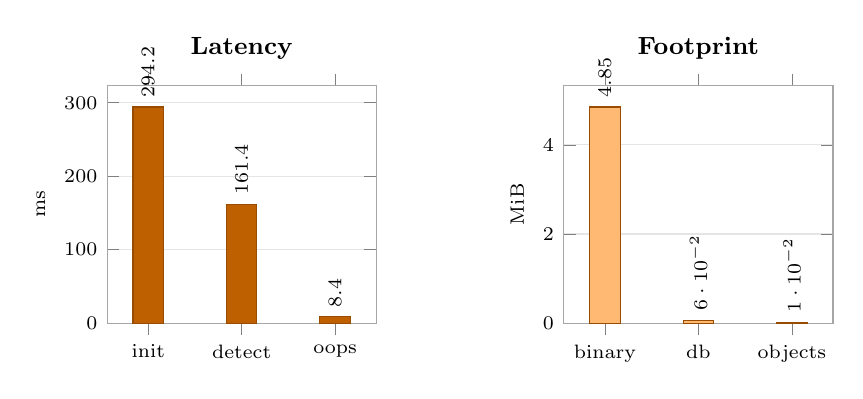
\begin{tikzpicture}
\begin{axis}[
    width=5.0cm,
    height=4.6cm,
    ybar,
    bar width=11pt,
    ymin=0,
    enlarge x limits=0.22,
    ylabel={ms},
    symbolic x coords={init,detect,oops},
    xtick=data,
    nodes near coords,
    every node near coord/.append style={font=\scriptsize, rotate=90, anchor=west},
    tick label style={font=\scriptsize},
    label style={font=\scriptsize},
    title={Latency},
    title style={font=\small\bfseries},
    axis line style={draw=black!35},
    ymajorgrids=true,
    grid style={draw=black!10},
]
\addplot[fill=orange!75!black, draw=orange!60!black] coordinates {
  (init,294.2)
  (detect,161.4)
  (oops,8.4)
};
\end{axis}
\begin{axis}[
    at={(5.8cm,0cm)},
    anchor=south west,
    width=5.0cm,
    height=4.6cm,
    ybar,
    bar width=11pt,
    ymin=0,
    enlarge x limits=0.22,
    ylabel={MiB},
    symbolic x coords={binary,db,objects},
    xtick=data,
    nodes near coords,
    every node near coord/.append style={font=\scriptsize, rotate=90, anchor=west},
    tick label style={font=\scriptsize},
    label style={font=\scriptsize},
    title={Footprint},
    title style={font=\small\bfseries},
    axis line style={draw=black!35},
    ymajorgrids=true,
    grid style={draw=black!10},
]
\addplot[fill=orange!55, draw=orange!60!black] coordinates {
  (binary,4.85)
  (db,0.06)
  (objects,0.01)
};
\end{axis}
\end{tikzpicture}
}
\caption{Synthetic-workload latency and footprint from the local micro-evaluation harness.}
\label{fig:microeval}
\end{figure}

\subsection{Rollback Case Study}

On the repo-snapshot workload, we also ran one explicit-session rollback case
using an attributed \texttt{codex} session. That session modified three real
project documents: \texttt{README.md}, \texttt{ARCHITECTURE.md}, and
\texttt{PHILOSOPHY.md}. A subsequent \texttt{au oops --confirm} restored all
three to their pre-session state, and the probe confirmed that the injected
marker text was gone afterwards. This is still artifact-level evidence, not a
human study, but it shows the intended session rollback path on real repository
files rather than toy fixtures.

\section{Related Work}

\subsection{Coding Agents and Developer Workflow Change}

Recent work documents the way increasing AI automation changes developer work
patterns, including delegation boundaries between humans and models and the
growing role of coding agents in development
workflows~\cite{chen2025codewithme,agarwal2026aiides}. AgentUndo sits at the
infrastructure layer beneath those studies: it is not another agent, but a
provenance and recovery substrate for environments where agents already write
code.

\subsection{Attribution of Model-Generated Code}

Attribution is emerging as an independent research problem for model-generated
code. Guo et al.\ study disentangled attribution of LLM-generated code through
code fingerprints~\cite{guo2026codefingerprints}. That line of work asks
``which model or generator likely produced this code?'' AgentUndo instead asks
``which local agent session wrote this file or line in this repository?'' The
former is a post hoc inference problem; the latter is a systems-capture
problem. They are complementary.

\subsection{Provenance and Time-Travel Systems}

The provenance community has long studied system-level capture and query layers.
Story Book demonstrated an extensible provenance framework for recording and
querying execution history~\cite{spillane2009storybook}. Pasquier et al.\
presented practical whole-system provenance capture with CamFlow, emphasizing
usable system-level provenance collection~\cite{pasquier2017practicalprovenance}.
AgentUndo borrows the mindset that capture should be a reusable substrate, but
scopes it to the developer workstation and to project file history rather than
whole-system causal graphs.

Time-travel debugging provides another useful analogy. Thiede et al.\ propose an
object-centric time-travel debugger for navigating recorded states over
time~\cite{thiede2023objectcentric}. AgentUndo shares that temporal intuition,
but targets repository file state rather than runtime object state.

\section{Limitations and Future Work}

The current prototype has several important limitations.

\begin{itemize}
  \item \textbf{Evaluation gap.} The system does not yet provide measured CPU,
  overhead under realistic long-running workloads.
  \item \textbf{Attribution gap.} Explicit hook-based attribution is strong
  where implemented, but process heuristics remain best-effort.
  \item \textbf{Scope gap.} The current artifact focuses on local files, not
  terminal side effects, database mutations, network effects, or remote agent
  actions.
  \item \textbf{Human factors gap.} We have not yet measured whether developers
  prefer session-scoped rollback and blame compared with editor-local recovery.
\end{itemize}

The next evaluation phase should include:

\begin{enumerate}
  \item microbenchmarks for watcher overhead and snapshot latency,
  \item storage-growth experiments under realistic edit bursts,
  \item attribution-accuracy tests across multiple editors and agents,
  \item a small user study or field deployment with real coding sessions,
  \item failure-mode analysis for concurrent writes and out-of-band edits.
\end{enumerate}

\section{Conclusion}

AI coding agents create a new class of local state-management problem: the
system must preserve a history of \emph{agent action} even when no human commit
boundary exists yet. AgentUndo is a concrete response to that shift. It treats
agents as processes that deserve continuous capture, explicit attribution, and
reversible rollback. The current artifact is best understood not as a finished
product or finished evaluation, but as a working prototype of a new systems
layer. In that sense, the central claim of this paper is modest but important:
source control is no longer enough by itself; agentic software engineering
needs a provenance-and-rollback substrate of its own.

\bibliographystyle{plain}
\bibliography{bibliography}

\end{document}
